%======================================================================
\subsection{BW-PDM-13 --- Plan: the vault file browser (1 Nov 2026)}\label{sec:pdm13-plan}
%======================================================================

\begin{epic}{PDM-13}{Vault file browser}{M3}{\stTodo}{(new, 1 Nov)}
Make the Files tab a browser you can read at a glance. Every file gets its own row, with an icon for its type. A
navigation pane lists projects, saved views and categories. A preview pane shows the model in 3D, its ISO picture,
its drawing sheets and its drawing package, plus what it uses, where it is used and its history. The ISO picture and
a light preview mesh are made off screen every time a file is saved.
\end{epic}

\paragraph{Why.} On 1 Nov you looked for the VL-P01 turbojet in the Files tab (figure~\ref{fig:pdm13-today}) and
could not find it: ``Why don't I have just an assembly of the turbojet?'' You asked for a part icon and an assembly
icon (``drawings should have an icon too''). You asked for a layout that is easier to read, like other PDM software,
with ``a preview pane of the 3D ISO, drawing packages, better navigation so I can find what I am looking for''. You
also said ``creating the 3D ISO should be part of the save feature (do it headless so the user doesn't see)'' and
asked ``is it possible to have a 3D view in the preview too?''

\paragraph{Your answers (1 Nov).}
\begin{itemize}[nosep]
  \item \textbf{Layout:} ``It should be by assemblies. Only top-line assemblies. Example: test stand contains engine
        but both show up. Everything should have a top line. Let's drop the drill down. I don't think PDM software
        does it that way.'' So the list is flat: every file is one row. What an assembly uses and where a file is
        used move to the preview pane.
  \item \textbf{The turbojet's structure stays as it is.} The test stand keeps the engine inside it; both get their
        own row.
  \item \textbf{The look:} the mockup in figure~\ref{fig:pdm13-mockup}, made from the real vault (``this is a good
        look to start with'').
  \item \textbf{Who builds it:} the Vector Labs session, in this repository, after this plan.
  \item \textbf{Assemblies reference parts; the CAD stays as it is:} ``It should be a file list. But the assemblies
        reference the parts in the vault. Like commercial softwares do.'' The rotor assembly stays a separate file that
        references the same parts as the engine; the browser shows those references in \emph{Uses} and
        \emph{Where used}.
  \item \textbf{Saves that make the picture and mesh:} files in a vault work folder only. Other files save exactly as
        FreeCAD does today.
  \item \textbf{Where the mesh lives:} inside the \file{.FCStd}, so it travels with every version and copy.
  \item \textbf{Drawing packages:} a PDF of each drawing, with WIP drawings included and watermarked. ``Allow me to
        build packages too'': you pick the files and the package is made from them (C, \emph{Build package}).
\end{itemize}

\begin{figure}[!htbp]
\centering
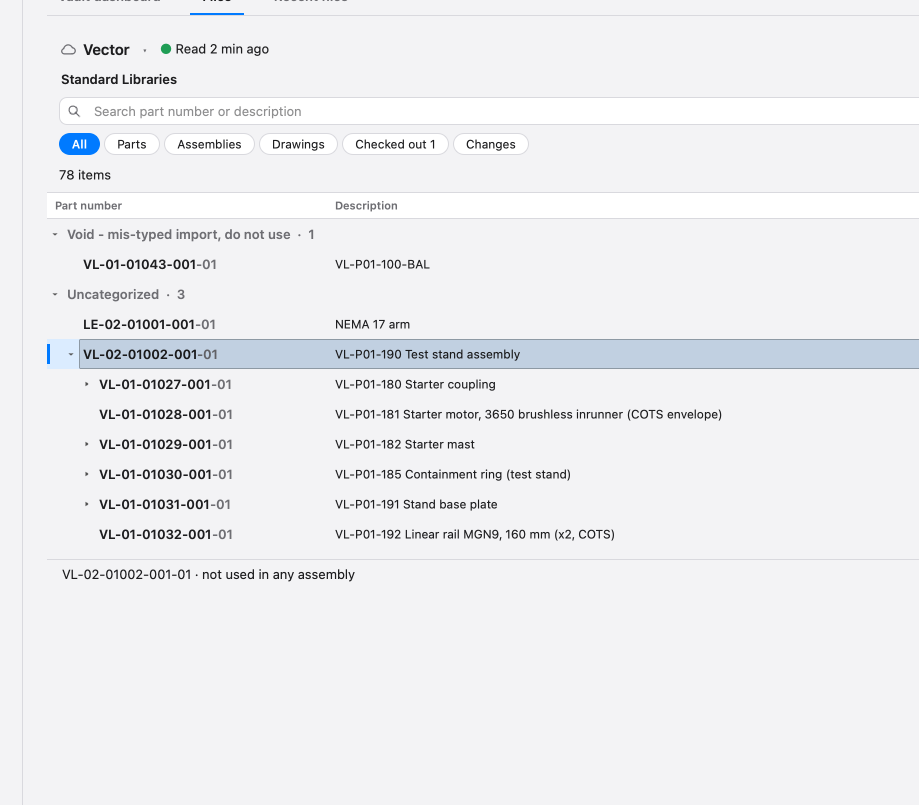
\includegraphics[width=0.62\linewidth]{fig/pdm13_today.png}
\caption{The Files tab today (1 Nov), with the \emph{Vector} vault open. The tree's roots are the assemblies that no
other assembly uses. The engine (\code{VL-02-01001-001}) sits inside the test stand, so it has no row of its own,
and the tree had to be opened to find it. No row shows its type.}
\label{fig:pdm13-today}
\end{figure}

\begin{figure}[!htbp]
\centering
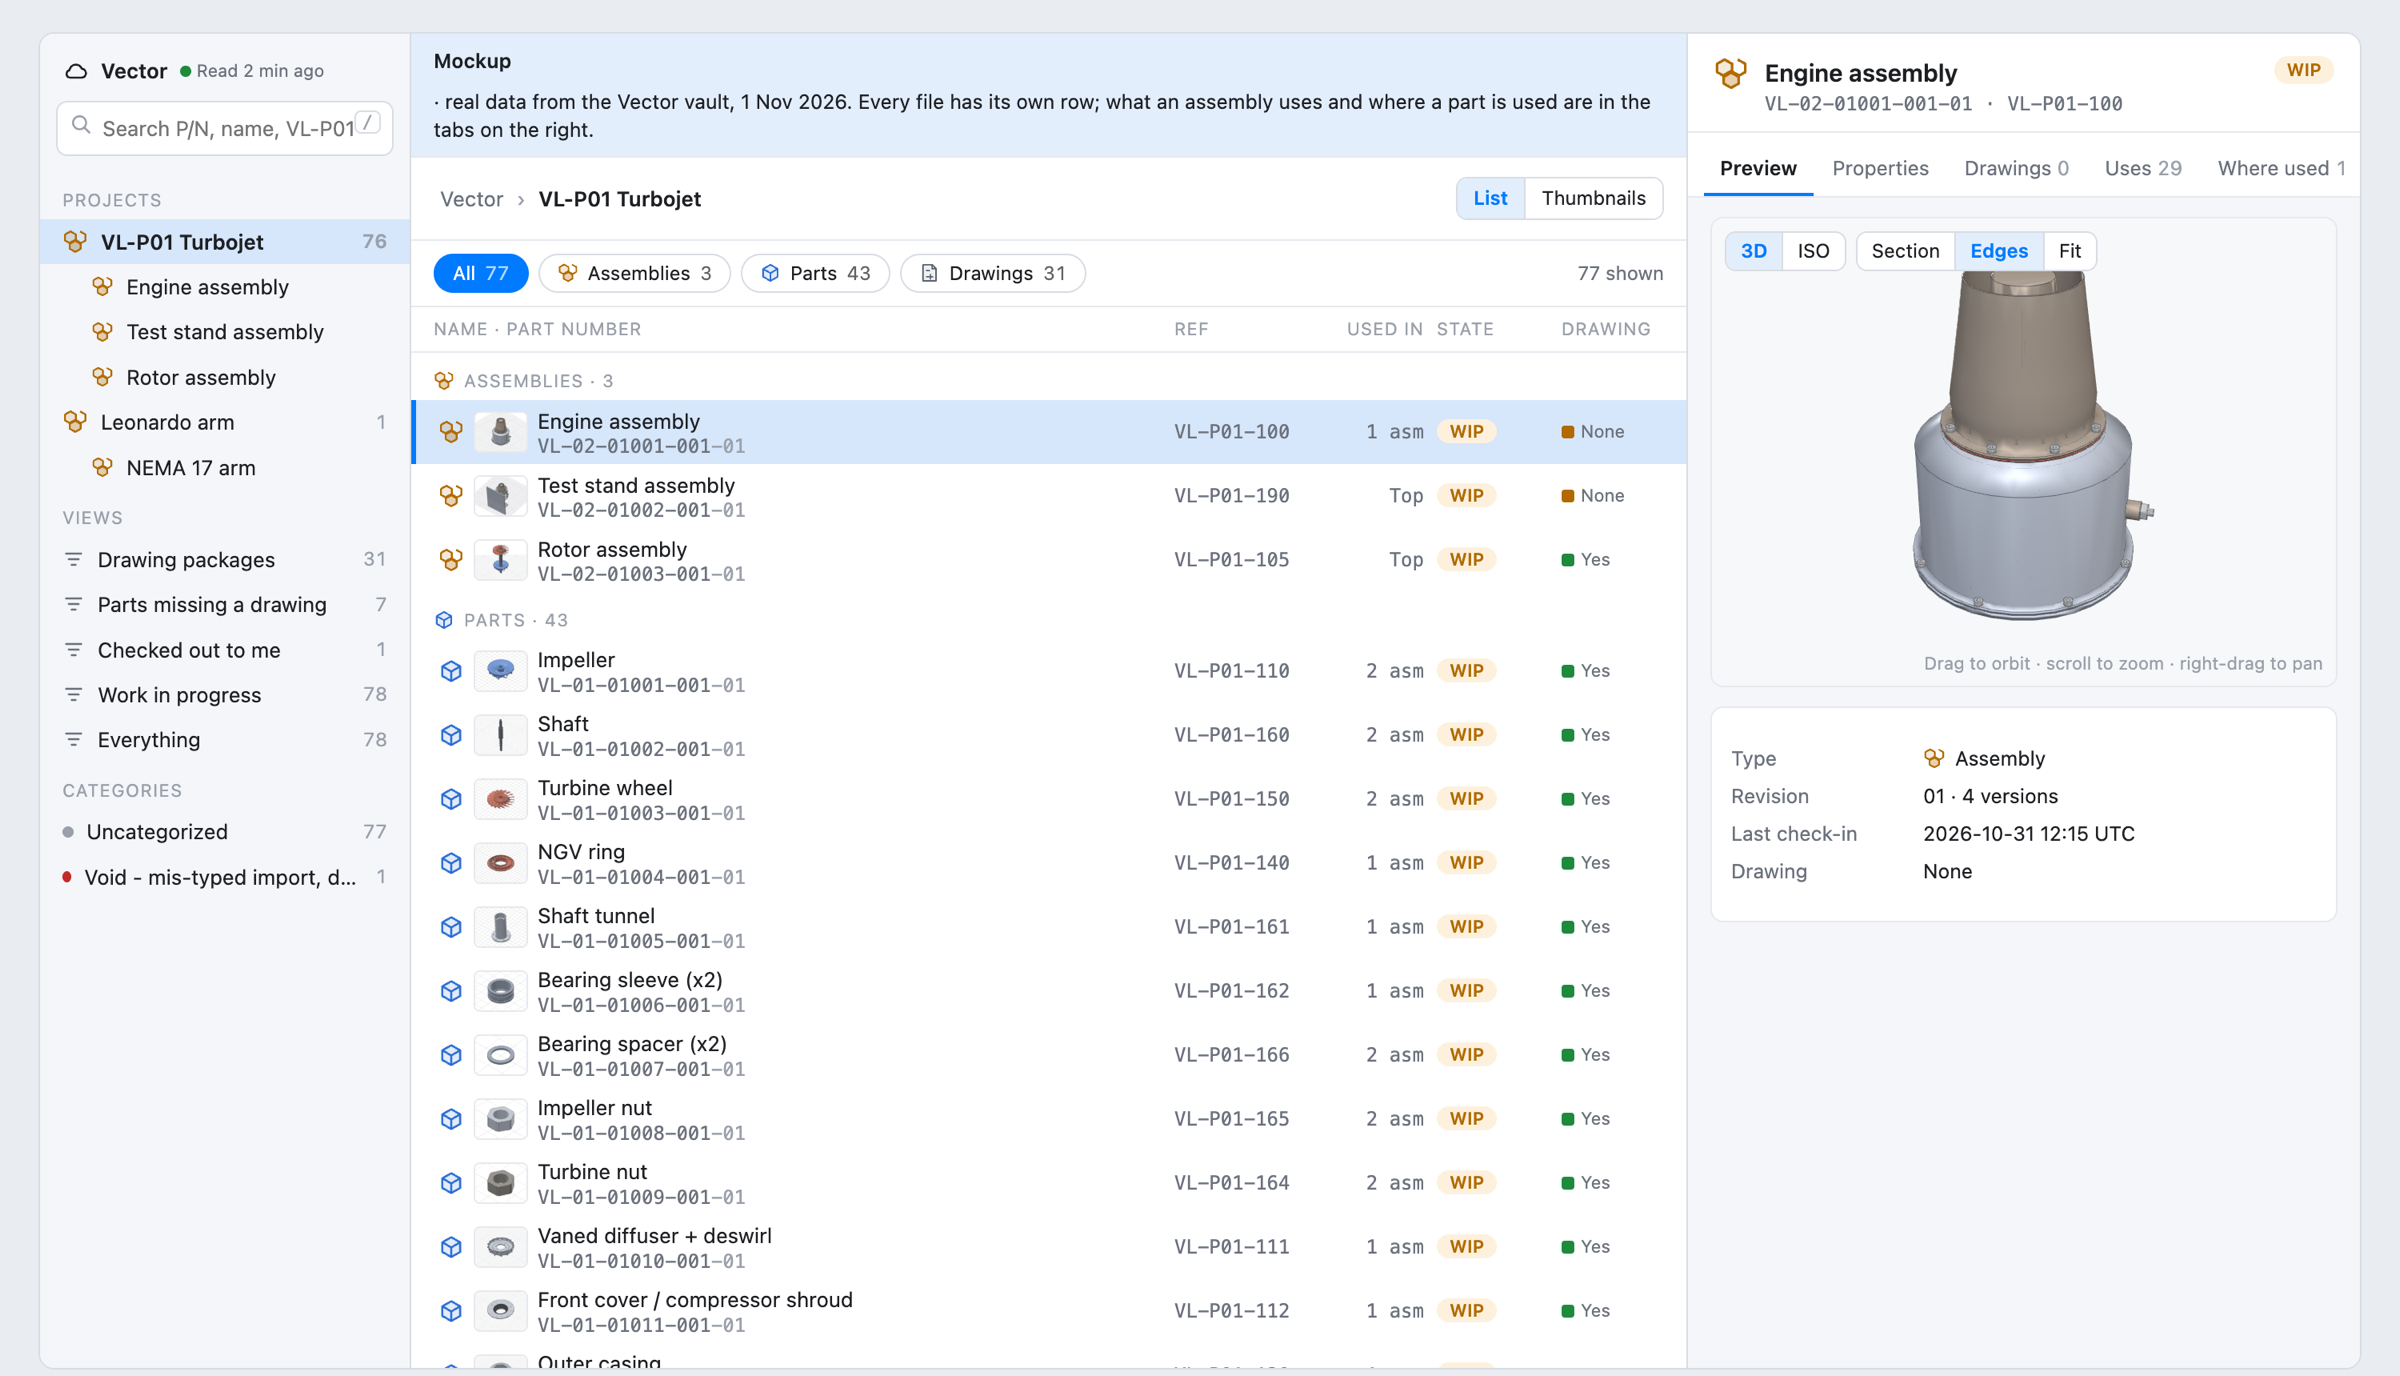
\includegraphics[width=\linewidth]{fig/pdm13_mockup.png}
\caption{The mockup Bruce approved as the starting look (\url{https://claude.ai/artifact/QXkDfmk7k84wa7T9VsM5zq}).
It shows the 77 items of the \emph{Vector} vault with their real thumbnails, drawings and check-in history. Left:
projects, views, categories. Middle: one row per file, grouped as assemblies, parts and drawings, each with its type
icon, thumbnail, P/N and revision, design ref, how many assemblies use it, state and drawing status. Right: the
selected file, here the engine in a live 3D view, with tabs for Properties, Drawings, Uses, Where used and History.}
\label{fig:pdm13-mockup}
\end{figure}

%----------------------------------------------------------------------
\subsubsection*{1. What I found (1 Nov)}

These findings come from the \emph{Vector} vault, read with \code{vault\_trees.structure} and \code{FolderVault}
(read only). The timings are off-screen runs of \file{build/release/bin/FreeCAD} on copies of the 46 turbojet model
files, under a throwaway profile.
\begin{enumerate}[nosep]
  \item \textbf{The tree hides top assemblies inside other ones.} \code{vault\_trees.tops} keeps only the assemblies
        that no BOM uses. The test stand (\code{VL-P01-190}) links the engine, so the engine is reachable only by opening
        the test stand. The rotor assembly (\code{VL-P01-105}) is a separate root, although the engine links the same
        six rotor parts directly. A part used in two assemblies is listed twice. Where it is used is only shown by
        tinting the other rows.
  \item \textbf{Nothing shows a file's type.} Parts, assemblies and drawings look the same; only the document-type
        digits of the P/N (01, 02, 03) tell them apart.
  \item \textbf{The turbojet's thumbnails are not ISO pictures.} The ISO picture (\file{bruceworx\_preview.py}) is
        made only by the GUI's check-in. The turbojet was checked in from a script (\code{vault\_sync.py}), so its
        files keep the thumbnail FreeCAD saved: the view from above. Every drawing's thumbnail is blank.
  \item \textbf{Drawing gaps.} The engine and test stand assemblies have no drawing. Seven parts have none (COTS
        envelopes excluded). The browser should make this visible without opening anything.
  \item \textbf{Off-screen work is cheap.} Over the 46 files (table below): an ISO picture takes 80\,ms (99\,ms
        at most), a part's preview mesh 3\,ms (0.5\,s for a whole assembly meshed in one piece, which instancing
        avoids), and writing the picture into the file takes 1\,ms (0.25\,s at most, for a 2.2\,MB file).
\end{enumerate}

\begin{center}
\footnotesize
\begin{tabularx}{\linewidth}{@{}>{\raggedright\arraybackslash}p{6.4cm}rrX@{}}
\toprule
Step, per file (46 turbojet files) & median & max & largest case\\
\midrule
Open the document (GUI) & 83\,ms & 1.75\,s & test stand, with every linked part\\
ISO picture, 512\,px, off screen (\code{bruceworx\_preview.render}) & 80\,ms & 99\,ms & impeller\\
Preview mesh, one part & 3\,ms & 0.5\,s & engine meshed whole (instancing avoids it)\\
Write the picture into the \file{.FCStd} (\code{set\_thumbnail}) & 1\,ms & 254\,ms & 2.2\,MB file\\
ISO picture size (PNG) & 12\,kB & & \\
\bottomrule
\end{tabularx}
\end{center}

%----------------------------------------------------------------------
\subsubsection*{2. How other PDM software does it}

\begin{center}
\small
\begin{tabularx}{\linewidth}{@{}>{\raggedright\arraybackslash}p{2.6cm}X@{}}
\toprule
Product & The file list and the pane under or beside it\\
\midrule
SOLIDWORKS PDM & Folder tree on the left; a flat file list with type icons, state and version columns; a pane with
  the tabs \emph{Preview}, \emph{Data Card}, \emph{Version}, \emph{Bill of Materials}, \emph{Contains} and
  \emph{Where Used}. Since 2024 SP2 the preview can sit on the right.\\
Autodesk Vault & Navigation pane (folders, saved searches); a flat main grid with icons, state and revision; a preview
  pane with \emph{Preview}, \emph{History}, \emph{Uses}, \emph{Where Used} and \emph{View} (a lightweight 3D or
  drawing viewer).\\
Onshape & Documents with thumbnails; inside, one tab per part studio, assembly or drawing; release management pulls an
  item's drawings into the release with it.\\
\bottomrule
\end{tabularx}
\end{center}
All three list files \emph{flat}: an assembly is one row, and the structure is a tab of the selected file. That is
the layout you chose. Sources: help.solidworks.com (\emph{Explorer Tabs}, \emph{File Detail View}),
help.autodesk.com (\emph{View File Details and History}), cad.onshape.com (\emph{Typical release workflow}).

%----------------------------------------------------------------------
\subsubsection*{3. The design}

\paragraph{A. The list.} One row per vault item, whatever uses it. The rows are grouped as \emph{Assemblies},
\emph{Parts} and \emph{Drawings}, in that order. Each group header carries its count and folds closed. A row shows:
the type icon (part: a blue cube; assembly: amber stacked cubes; drawing: a grey sheet), the thumbnail, the name
(the description without its design ref) over P/N-REV, the design ref (\code{VL-P01-110}), \emph{Used in} (``2 asm'',
``Top'' for an assembly nothing uses), the state chip, the drawing status (Yes / None / COTS) and today's status
column (lock, Get latest). There is no expand arrow anywhere. The chips stay (All, Assemblies, Parts, Drawings,
Checked out, Changes), each with its count. Sorting by part number or by time modified stays. The categories group
the list as today (\S\ref{sec:pdm09-plan}, categories built), with the type groups inside each.
\textbf{Replaces:} \code{vault\_trees.file\_tree} as the list's source; \code{file\_tree}, \code{tops} and the
\emph{Not in an assembly} group stay for the dashboard's projects.

\paragraph{B. Navigation.} A pane at the left of the Files tab, folding to icons when the Start page is narrow.
\begin{itemize}[nosep]
  \item \textbf{Projects:} each program (VL, LE, OW, \ldots, named from \file{numbering.json}) with its item count.
        Under it, every assembly of the program. Clicking an assembly shows it and everything it uses, at any depth,
        as flat rows.
  \item \textbf{Views:} \emph{Drawing packages}, \emph{Parts missing a drawing}, \emph{Checked out to me},
        \emph{Work in progress}, \emph{Everything}. Each is a saved filter with a live count.
  \item \textbf{Categories} as today, with show/hide.
  \item \textbf{Breadcrumbs} over the list (Vector \textrangle{} VL-P01 Turbojet \textrangle{} Engine assembly and
        its contents). \textbf{Search} finds P/N, former numbers, name, design ref and state; \code{/} focuses it and
        \code{Esc} clears it. The arrow keys move through the rows, and Return opens the file.
\end{itemize}

\paragraph{C. The preview pane.} On the right of the list (below it when the Start page is narrow). The header is the
selected file's icon, name, P/N-REV, design ref and state. The tabs are:
\begin{itemize}[nosep]
  \item \textbf{Preview:} a switch between \emph{3D}, \emph{ISO} and \emph{Drawing}.
        \emph{3D} is a live viewer: orbit, zoom, pan, fit, a section cut on a mid plane, edges on or off. It draws
        the file's preview mesh (D), not the document, so nothing opens and nothing on screen moves. \emph{ISO} is the
        saved picture. \emph{Drawing} is the first sheet of the file's drawing, or of the drawing itself.
        Under the viewer: type, revision and versions, last check-in, drawing.
  \item \textbf{Properties:} the data card. P/N, revision, name, design ref, type, state, category, project, who
        has it checked out, file.
  \item \textbf{Drawings:} the drawing package. Each drawing of the file, with its sheet and its state. \emph{Export
        package} writes one PDF per drawing into a folder you pick: released drawings as they are, WIP drawings with an
        \emph{IN PROGRESS} watermark across each sheet. For an assembly the package holds the drawings of the assembly
        and of every file it uses, at any depth.
  \item \textbf{Build package} (your own packages): select any rows in the list (Shift and Command extend the
        selection), right-click, \emph{Build Package\ldots}. A dialog lists the drawings that come with them, each with
        its state; you untick what you don't want, name the package and pick the folder. A package is a folder of PDFs
        plus \file{package.csv} (P/N, revision, state, sheet file), so a supplier sees what is released. The vault
        records nothing; a package is a copy for sending.
  \item \textbf{Uses} (assemblies): the BOM lines, with quantities. Clicking one selects that row.
  \item \textbf{Where used:} the assemblies that use the file, with quantities.
  \item \textbf{History:} every version, newest first, with its comment, time, who checked it in and its size.
\end{itemize}

\paragraph{D. The ISO picture and the preview mesh, made at every save.} When a document is saved
(\code{slotFinishSaveDocument}, which \file{bruceworx\_vaultclient.py} already observes), a short timer after the save
returns:
\begin{enumerate}[nosep]
  \item renders the ISO picture off screen with \code{bruceworx\_preview.render}. The views on screen do not move;
        the user sees nothing.
  \item tessellates each part's shape into the preview mesh (E). For an assembly, it records each link's P/N and
        placement instead of meshing the parts again.
  \item writes both into the saved file: the picture as \file{thumbnails/Thumbnail.png} (marked as ISO, as today), the
        mesh as \file{bruceworx/preview.bin}. FreeCAD rewrites the archive at the next save, so they are written again
        every time.
\end{enumerate}
The check-in's own stamping (\code{stamp\_work\_file}) stays, for files saved before this existed. \emph{Refresh
Pictures} also makes the meshes, so the turbojet's 46 files get both without a new version.

\paragraph{E. The preview viewer.} A widget inside the pane that draws the file's preview mesh with Coin, through
the same off-screen renderer as the ISO pictures (\code{SoQtOffscreenRenderer}), and shows each frame as an image.
pivy's \code{QuarterWidget} was the first choice; in this build it cannot import its GL widget, and with that
patched in it crashes on GL errors (spike, 1 Nov). A frame of the engine (162\,000 triangles) at
800\,$\times$\,600 takes 50\,ms, so dragging redraws at about 20 frames a second at screen resolution and
sharpens when the mouse stops. Lighting follows the camera, as in the ISO pictures. Each part is one
\code{SoIndexedFaceSet} with its colour; an assembly's instances share their part's node through
\code{SoMatrixTransform}. The section is an \code{SoClipPlane} through the centre that keeps the far half, so the
cut face looks at you. A file without a preview mesh shows a note and a \emph{Make Previews} button.

%----------------------------------------------------------------------
\subsubsection*{4. Theory}

\paragraph{How fine the preview mesh is.} A curved face of radius $r$ cut into chords of angle $\theta$ deviates from
the true surface by the sagitta $s = r(1-\cos\tfrac{\theta}{2}) \approx r\theta^2/8$. The mesher takes a linear
deflection $\delta$ (the largest $s$) and an angular deflection $\theta_{\max}$, so each circle gets
\[
  n(r) = \max\!\left(\frac{2\pi}{\theta_{\max}},\ \frac{2\pi}{2\arccos(1-\delta/r)}\right)
       \approx \max\!\left(\frac{2\pi}{\theta_{\max}},\ \pi\sqrt{\frac{r}{2\delta}}\right)
\]
segments. The preview does not need a part's tolerances; it needs the part to look round in a pane about 400\,px
wide. Taking $\delta = 0.004\,D$ ($D$ the part's bounding-box diagonal, at least 0.05\,mm) and $\theta_{\max} =
0.35$\,rad gives every circle at least 18 segments. A circle whose diameter is the whole part gets
$\pi\sqrt{0.5D/(2 \cdot 0.004D)} \approx 25$. On screen that is an error of $0.004 \times 400 \approx 1.6$\,px at most,
and well under a pixel on most faces. Measured on the turbojet: \textbf{132\,188 triangles for all 43 parts}, the
largest part 18\,800 (outer liner), and 2.0\,MB in total (base64 text; about 1.5\,MB in binary).

\paragraph{Why assemblies are instanced.} With $P$ unique parts of $t_p$ triangles and $k_p$ instances each, meshing
every assembly as one shape costs $\sum_p k_p t_p$ triangles per assembly, again for each assembly that contains it.
Instancing stores $\sum_p t_p$ once, plus 16 numbers per instance. For the turbojet's three assemblies, meshing each as
one shape gave 299\,000 triangles; instanced they need no new triangles at all, only 102 placements (6.5\,kB). All
placements were checked: each instance's box centre matches the CAD to 0.000\,mm.

\paragraph{What a save costs.} The extra time per save is
$t = t_\text{ISO} + t_\text{mesh} + t_\text{write} \approx 80 + 3k + 1$\,ms for a part ($k$ shapes), and about
$100$\,ms for an assembly. It runs after the save has returned. Off-screen rendering needs the GUI thread's GL context,
so the window is busy for that tenth of a second. FreeCADCmd has no GL, so a headless save (a script, \code{vault\_sync})
writes only the mesh; the picture follows at the next GUI save or \emph{Refresh Pictures}.

%----------------------------------------------------------------------
\subsubsection*{5. Steps}

\begin{enumerate}[nosep]
  \item \textbf{Flat list and type icons} (\file{bruceworx\_vaultclient.py}, \file{vault\_trees.py}): rows grouped by
        type, the three icons in the SVG set, \emph{Used in} and \emph{Drawing} columns, no expanders. Tests: every item
        one row; the group order; counts per chip; \emph{Used in} against the BOMs; the turbojet vault copy (engine and
        test stand both listed).
  \item \textbf{Navigation pane}: projects with their assemblies, views, categories, breadcrumbs, keyboard. Tests:
        each view's filter and count; an assembly's contents at any depth; search by former number.
  \item \textbf{Preview pane}: tabs, data card, Uses / Where used / History, drawing package, ISO and drawing previews.
        Tests: each tab on a part, an assembly, a drawing, a COTS part and an item with no file.
  \item \textbf{Preview mesh} (new \file{bruceworx\_previewmesh.py}, FreeCAD-free reader and writer; a GUI-free
        tessellator): the format, written by \emph{Refresh Pictures}, and by the save hook. Tests: round trip; the
        instance placements against \code{Shape.BoundBox}; a damaged entry falls back to the ISO picture.
  \item \textbf{3D viewer} (off-screen frames, E): orbit, zoom, pan, fit, section; one widget reused. Tests: off-screen
        render of the engine, rotor and test stand compared with the ISO picture's silhouette.
  \item \textbf{Save hook}: ISO picture and mesh after every save, for vault work files only. Tests: the picture
        and the mesh are in the saved file; no view moved; a save outside the vault (if chosen); a 2\,MB assembly
        under 0.3\,s.
  \item \textbf{Turbojet}: \emph{Refresh Pictures} on the \emph{Vector} vault (cache only), then the next check-in
        of each file carries its picture and mesh.
\end{enumerate}

%----------------------------------------------------------------------
\subsubsection*{6. Decided while planning}

\begin{itemize}[nosep]
  \item \emph{Parts missing a drawing} becomes \emph{Missing a drawing} and counts assemblies too (the engine and the
        test stand have none). COTS envelopes are left out.
  \item STEP and DXF are not in the default package; \emph{Build package} can add them later if you ask.
  \item No questions are open. Building starts with step~1.
\end{itemize}

%----------------------------------------------------------------------
\subsubsection*{7. Built (1 Nov 2026)}

\begin{figure}[!htbp]
\centering
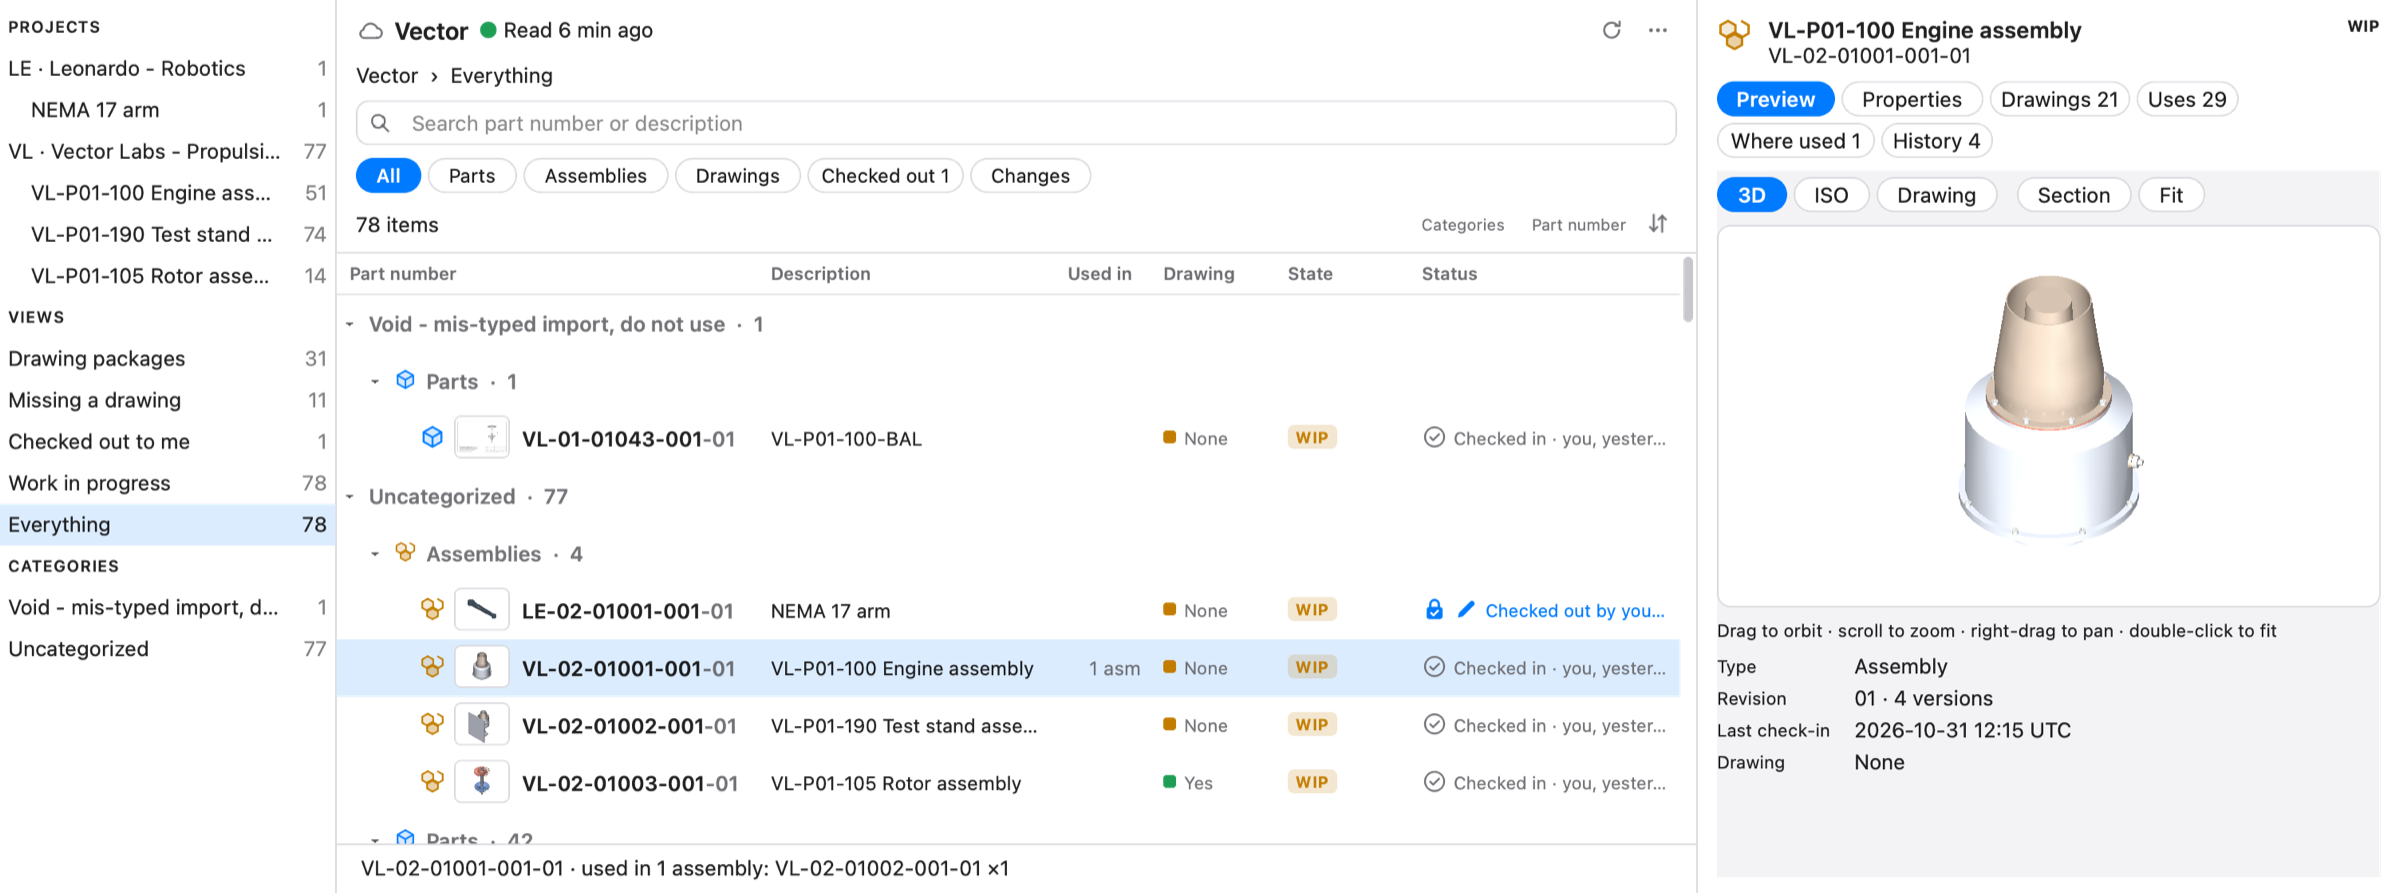
\includegraphics[width=\linewidth]{fig/pdm13_built_files.png}
\caption{The Files tab as built, on a copy of the \emph{Vector} vault: projects with their assemblies, views and
categories at the left; one row per file, grouped by type, with icon, picture, Used in and Drawing; the engine in 3D
at the right with its tabs.}
\label{fig:pdm13-built}
\end{figure}

\begin{figure}[!htbp]
\centering
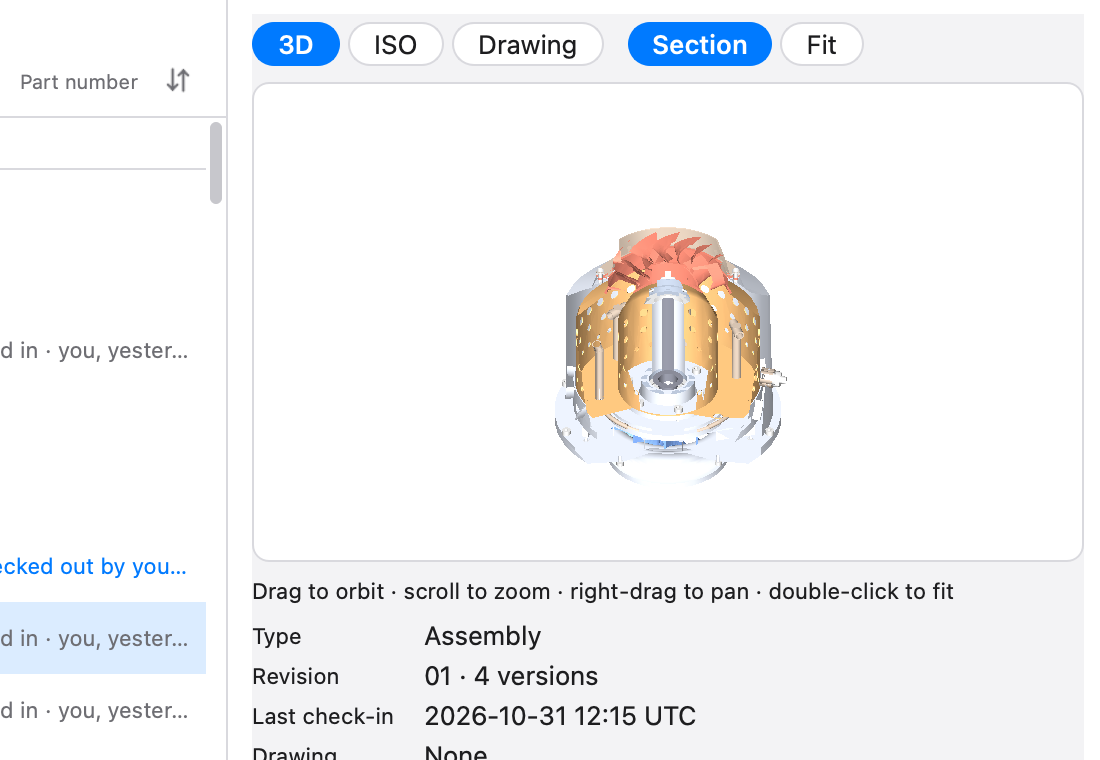
\includegraphics[width=0.48\linewidth]{fig/pdm13_built_section.png}\hfill
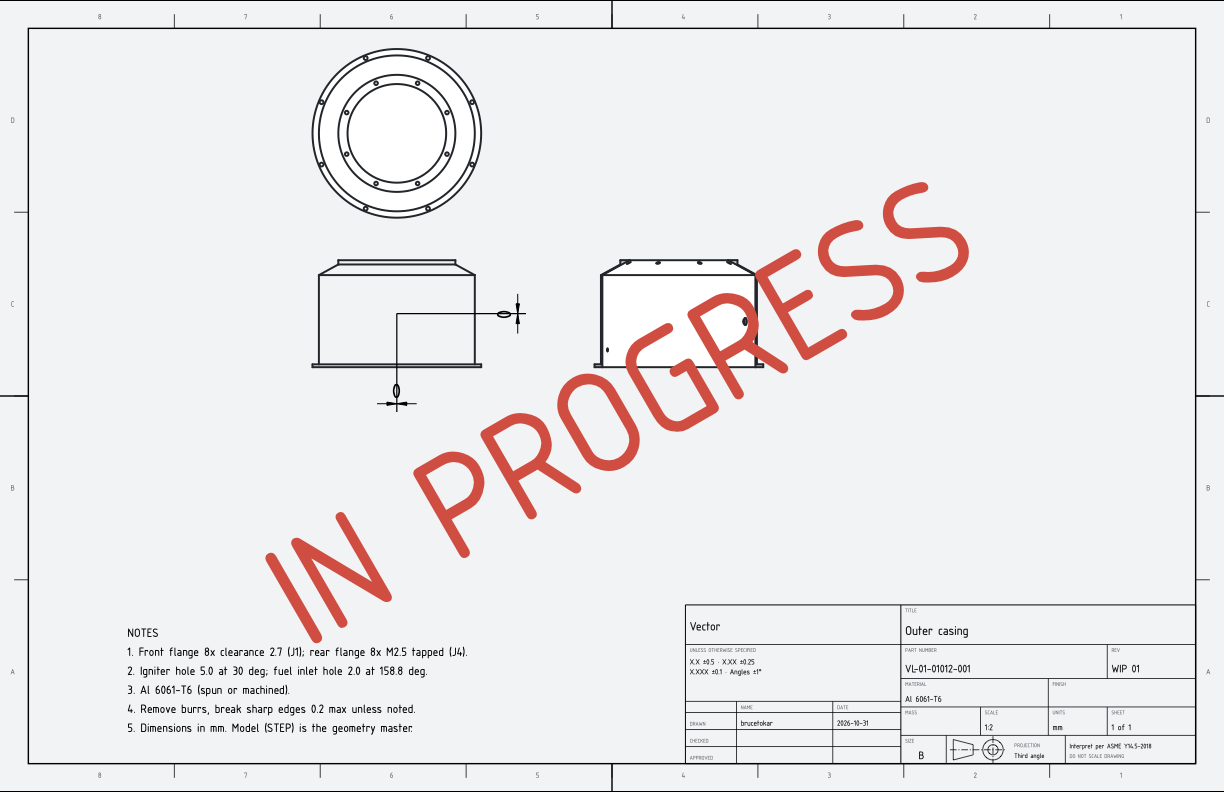
\includegraphics[width=0.48\linewidth]{fig/pdm13_built_package.png}
\caption{Left: the engine's section in the preview, through its centre and square to the view. Right: a sheet
of a built package, the outer casing drawing, WIP and therefore stamped IN PROGRESS.}
\end{figure}

\paragraph{What you can do now.}
\begin{itemize}[nosep]
  \item Find any file in one row: every assembly, part and drawing has its own line, under Assemblies, Parts or
        Drawings, with its type icon and picture. The engine and the test stand both have rows.
  \item Pick a project, one of its assemblies (it shows itself and everything it uses), a view or a category on
        the left. The breadcrumb says where you are.
  \item Select a file to see it in 3D without opening it: drag to orbit, scroll to zoom, right-drag to pan,
        double-click to fit, \emph{Section} to cut it through the centre. \emph{ISO} shows its picture,
        \emph{Drawing} its first sheet. The tabs show its properties, drawings, what it uses, where it is used and
        its history.
  \item Save a vault file and its ISO picture and preview mesh are written into it; a drawing gets the picture of
        its sheet. \emph{Make Previews} does this for files saved before, into the cache on this Mac.
  \item Right-click one or more rows, \emph{Build Package\ldots}, or \emph{Export Package\ldots} in the Drawings tab:
        a PDF of each drawing, WIP ones stamped IN PROGRESS, and \file{package.csv}.
\end{itemize}

\paragraph{Decided while building.}
\begin{itemize}[nosep]
  \item \textbf{The 3D view draws its own frames.} pivy's \code{QuarterWidget} cannot import its GL widget in this
        build and crashes with it patched in. The view renders with \code{SoQtOffscreenRenderer} (50\,ms a frame for
        the engine at 800\,$\times$\,600) and shows the image. That renderer ignores Coin clip planes and sets its own
        near plane, and keeps what it drew of a scene, so the section drops the triangles in front of the cut
        (numpy, 15\,ms for the engine) and every new scene gets a new renderer.
  \item \textbf{A search counts matches.} A category or type group shows how many rows match, not how many the
        category holds.
  \item \textbf{An instance in another vault is left out of the 3D view.} The NEMA 17 arm links its motor from
        Standard Libraries; the preview shows the arm only. Following links across vaults is a later step.
  \item \textbf{Make Previews is slow for drawings.} A drawing opened hidden waits for TechDraw to compute its views,
        about 11\,s a sheet, so the first Make Previews on the \emph{Vector} vault (77 files, 31 drawings) took
        6 minutes. A drawing saved in the GUI gets its picture at once.
\end{itemize}

\paragraph{Tests.} \file{TestBruceWorxVaultBrowser.py} (12), \file{TestBruceWorxPackage.py} (5),
\file{TestBruceWorxPreviewMesh.py} (7), \file{TestBruceWorxPreview.py} (12), \file{TestBruceWorxVaultClient.py}
(38, the category test updated) and the addon's \file{test\_vault\_trees.py} (14): all pass. Off screen on a
copy of the vault: Make Previews for 77 files; the engine, turbine and test stand in 3D; the section; a drawing
sheet; a package of three drawings (three PDFs and \file{package.csv}); a save of a checked-out assembly writing its
picture and mesh with the 3D view untouched.

\paragraph{Open.} \emph{Make Previews} on your own vault (it writes only to the cache on your Mac). The docs GUI test
\file{test\_vault\_work.py} still looks for the floating Vault card removed on 25 Oct; it needs a rewrite for the
Files tab.
